\documentclass[12pt, a4]{report}
\usepackage[utf8]{inputenc}
\usepackage[margin=0.8in]{geometry}
\def\thesection{\arabic{section}}
\setcounter{tocdepth}{4}
\usepackage{graphicx}
\graphicspath{ {images/} }
% Below are for the code blocks
\usepackage{listings}
\usepackage{courier}
\usepackage{verbatim}
\usepackage{color}
\usepackage{rotating}

% Below are table config
\setlength{\arrayrulewidth}{0.5mm}
\setlength{\tabcolsep}{10pt}
\renewcommand{\arraystretch}{1.5}

\definecolor{codegreen}{rgb}{0,0.6,0}
\definecolor{codegray}{rgb}{0.5,0.5,0.5}
\definecolor{codepurple}{rgb}{0.58,0,0.82}
\definecolor{backcolour}{rgb}{0.95,0.5,0.92}
\definecolor{bittersweet}{rgb}{1.0, 0.44, 0.37}
\definecolor{cosmiclatte}{rgb}{0.93, 0.93, 0.93}
\definecolor{eggshell}{rgb}{0.94, 0.94, 0.9}
\definecolor{fandango}{rgb}{0.71, 0.2, 0.54}

\lstdefinestyle{mystyle}{
	backgroundcolor=\color{cosmiclatte},   
	commentstyle=\color{codegreen},
	keywordstyle=\color{fandango}\small,
	numberstyle=\tiny\color{codegray},
	stringstyle=\color{codepurple},
	basicstyle=\ttfamily\footnotesize,
	breakatwhitespace=false,        
	breaklines=true,               
	captionpos=b,                    
	keepspaces=true,  
	numbers=left,                    
	numbersep=5pt,                  
	showspaces=false,                
	showstringspaces=false,
	showtabs=false,                  
	tabsize=2
}

\lstset{style=mystyle}

\title{2810, Software Technologies Assignment 1}
\author{Zaymon Foulds-Cook, s5017391 \textbar{} Natnicha Titiphanpong, s2940970}%\thanks{}}
\date{\today}

\begin{document}

\begin{titlepage}
	\maketitle
\end{titlepage}
 \tableofcontents
\pagebreak
\section{Software Technologies Assignment 1}
\subsection{Problem Statement}
	\par 
	
\subsection{User Requirements}
	\textbf{The following list itemizes the user requirements for the implementation of the Ladder-gram program}
	\begin{itemize}
		\item The user should be able to interact with the program by specifying the dictionary file name$($without the .txt extension$)$
		\item The user should be able to interact with the program by specifying the source and target word.
		\item The user should be able to supply a list of words that cannot be used in the path solution by specifying the file name$($without the .txt extension$)$ and placing it in the same directory as the program file.
		\item The user will be displayed with the shortest path from source word to target word as the solution.
	\end{itemize}
	
\subsection{Software Requirements}
	\textbf{The following list itemizes the software requirements for the implementation of the Ladder-gram program}
	\begin{itemize}
		\item The program will notify the user if the inputs are invalid
		\item The program will notify the user if a solution was found
		\item If a valid solution is found the program will print it to the console
		\item The program will default to printing the shortest path to the console
		\item If the user chooses to input a list of banned words, the program will remove those words from the solution's list
		\item The program will report the length of the solution found 
	\end{itemize}
	\pagebreak
	
\subsection{Software Design}
	\subsubsection{High Level Design - Logical Block Diagram}

	\begin{figure}[!h]
	\centering
	\includegraphics[scale=0.6]{Logical_Block_Laddergram}
	\caption{Logical block diagram for the Python implementation of Ladder-gram}
	\end{figure}
				
	\pagebreak

	\subsubsection{Structure Chart - UML}
	\paragraph{}

	\begin{figure}[!h]
	\centering
	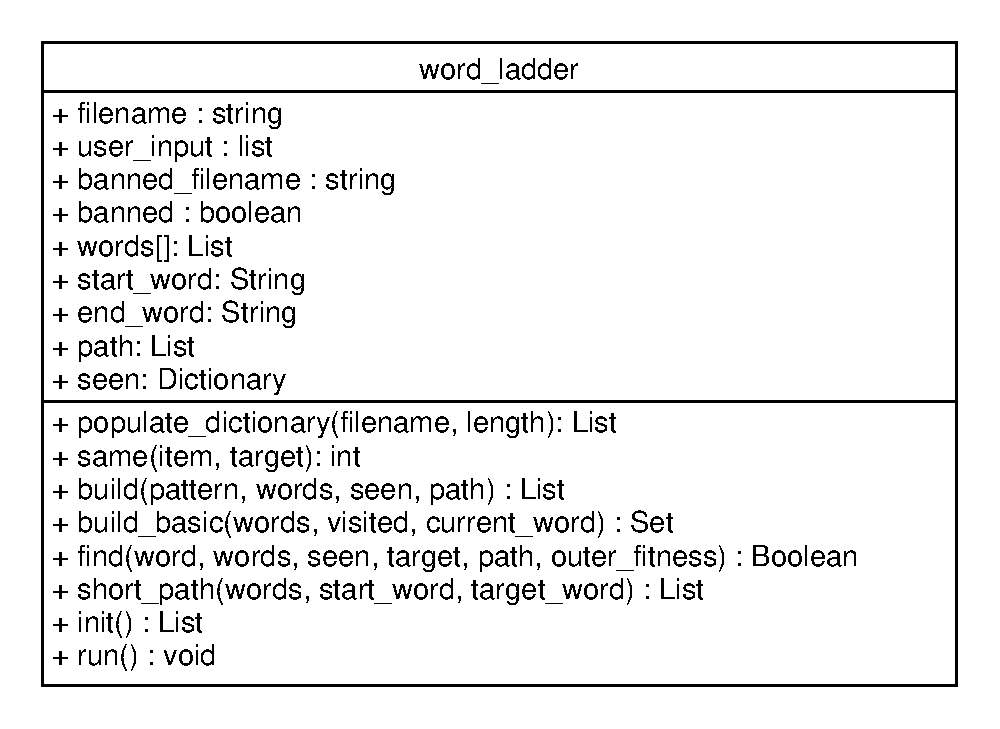
\includegraphics[scale=0.7]{UML}
	\caption{UML diagram for the Python implementation of Ladder-gram}
	\end{figure}


	\subsubsection{List all functions in the software}
	\textbf{	Functions in the Ladder-gram Program}
	\begin{enumerate}
		\item
			\textbf{populate\_dictionary}
			\textbar{}  Function that takes in a filename, a word length and a banned file name, returns a list that contains all words in the file of the specified length and ignoring words that occur in the banned words file.
			\par Input Parameters: filename, length, banned\_filename 
			\par Side Effects:
			\begin{itemize}
				\item Populate words list
			\end{itemize}
			\par Returns: List
		\item
			\textbf{same}
			\textbar{}  Function that determines how similar two words are by comparing characters in-place. Returns number of characters that are the same.
			\par Input Parameters: str1, str2
			\par Side Effects: None
			\par Returns: Integer
		\item
			\textbf{build}
			\textbar{}  Function that returns a list of all words that are one letter away from the last word in the path and have not been seen before.
			    Function also calculates the fitness of each word and adds it with the word in a tuple.
			\par Input Parameters: pattern $($regex pattern$)$, words, seen, path
			\par Side Effects: None
			\par Returns: List of tuples
		\item 
			\textbf{build\_basic}
			\textbar{} Similar to build function except it does not return a tuple with fitness of the word.  
			\par Input Parameters: words, visited, current\_word 
			\par Side Effects: None 
			\par Returns: Set of neighboring elements 
		\item
			\textbf{find}
			\textbar{}  Recursive function that finds a path from one word two another of the same length by going through intermediary words which are one character different.
			\par Input Parameters: word, words, seen, target, path, outer\_fitness
			\par Side Effects
			\begin{itemize}
				\item `Path' global variable gets modified 
				\item `Seen' global variable gets modified
			\end{itemize}
			\par Returns: Boolean
		\item
			\textbf{short\_path}
			\textbar{} Function that uses breadth-first search to find the shortest path of any given word pair. 
			\par Input Parameters: words, start\_word, target\_word 
			\par Side Effects: None
			\par Returns: Path 
		\item
			\textbf{init}
			\textbar{} Function that accepts user input and performs input validation.   
			\par Input Parameters: None  
			\par Side Effects: None
			\par Returns: List
		\item
		\textbf{Run}
		\textbar{} Function which wraps main method contents to allow the module to be runnable in system tests.
		\par Input Parameters: None  
		\par Side Effects: Sys.Stdout
		\par Returns: void
	
	\begin{comment}
			\item
				\textbf{}
				\textbar{}  
				\par Input Parameters:
				\par Side Effects
				\begin{itemize}
				\item 
				\end{itemize}
				\par Returns:
	\end{comment}
	
	\end{enumerate}
	\newpage
	
	\subsubsection{List all of the data structures in the Ladder-gram program}
		\par Finish this!
		\begin{enumerate}
				\item
					\textbf{Dictionary}
					\textbar{} Purpose
					\par Used in the following functions:
					\begin{itemize}
						\item find
						\item build
					\end{itemize}
				\item
					\textbf{List}
					\textbar{} Purpose
					\par Used in the following functions:
					\begin{itemize}
						\item find
						\item build
						\item populate\_dictionary
					\end{itemize}
				\item 
					\textbf{Set}
					\textbar{} Purpose 
					\par Used in the following functions:
					\begin{itemize}
						\item build\_basic
					\end{itemize}
				\item
					\textbf{Tuple}
					\textbar{} Purpose
					\par Used in the following functions:
					\begin{itemize}
						\item find
						\item build
					\end{itemize}
		\end{enumerate}
	
	\newpage 
	\subsubsection{Detailed Design}
	
	
	\textbf{Generate Solutions Pseudo-code}
	
	\begin{comment}
			\begin{figure}[h]
			\lstinputlisting[language=Python]{pseudocode_New.py}
			\caption{Psuedo-code for the generate solutions algorithm}
			\end{figure}
	\end{comment}

	
	\pagebreak
	\subsection{Configuration Management and Version Control}
		\par 
		The development of this program required the use of version control software to evenly distribute tasks, as well as monitor the changes through a log. GitHub was designed for users as a way to manage documents, programs and other information. GitHub was neccessary for sharing of files and the ability to compare files and identify differences and merge changes if needed prior to commit. Version control was used to ensure each developer could work on tasks individually as well, even after finishing a formal collaboration. The software records a log of past commits pushed to the repository which allows for backtracking of file versions.
	
	\subsection{Unit Test}


		\begin{tabular}{ |p{0.5cm}|p{5cm}|p{5cm}|p{5cm}| }
			\hline
			No. & Test Case & Expected Results & Actual Results \\
			\hline
			1.0 & \textbf{Test User Input} &  & \\
			1.1 & Input contains number: 1. & Program displays error message: ``Source or target input words cannot contain numbers or special characters" and system exits. & As expected.\\
			1.2 & Source or target input contains special character `@'. & Program displays error message: ``Input words cannot contain numbers or special characters" and system exits. & As expected. \\
			1.3 & Source or target input contains special character: `\_'. & Program displays error message: ``Input words cannot contain numbers or special characters" and system exits. & As expected. \\
			1.4 & Source or target input contains number: 3. & Program displays error message: ``Input words cannot contain numbers or special characters and system exits." & As expected. \\
			1.5 & Source and target words are the same & System prints error: ``Start and target words cannot be the same." & As expected. \\
			1.6 & Target word input is of different length to source word. & System prints error message: ``Start and target words must be the same length." & As expected \\
			1.7 & Check whether init function returns source and target word after input is validated & Function returns source word as the first element in the list and target as second. & As expected.\\
			2.0 & \textbf{Test Helper Functions} &  &  \\
			2.1 & Test same function and whether it returns the correct number of identical letters & Test case returns true if same function returns 4 for `lead' \& `lead', 3 for `lead' \& `mead' and false if `hello' \& `there' equals 0. & As expected. \\
			\hline
		\end{tabular}

			\pagebreak[4]
			
		\begin{tabular}{ |p{0.5cm}|p{5cm}|p{5cm}|p{5cm}| } 
			\hline
			No. & Test Case & Expected Results & Actual Results \\
			\hline
			2.2 & Test build basic function & All words that are adjacent to the start word and not visited in dictionary, are in the list returned by the function. Checks correctness of function with and without keys in visited dictionary. & As expected. \\
			2.3 & Test build function & Builds the list of neighboring elements correctly by returning a list with no words that have been seen or are in the current path.  & As expected\\
			2.4 & Test populate dictionary function & Reads in dictionary filename and checks the correct number of words present for each word length & As expected. \\
			2.5 & Test populate dictionary function takes list of banned words & Reads in banned words list, and asserts that banned words are not present in the populated lists. & As expected. \\
			3.0 & \textbf{System tests} &  &  \\
			3.1 & Test full system using recursive algorithm with mock input & Reads in required input and outputs a valid path from start to target word & As expected. \\
			3.2 & Test full system using breadth-first search with mock input & Reads in required input and outputs the shortest path from start to target word & As expected. \\
			\hline
		\end{tabular}
	\newpage
	\subsection{Requirement Acceptance Test}
	
		\begin{tabular}{ |p{0.5cm}|p{7.25cm}|p{2.5cm}|p{2.5cm}|p{2cm}| }
			\hline
			No. & Test & Implemented (Full/Partial/None) & Test Results (Pass/Fail) & Comments \\
			\hline
			1 & The program will be able to read in the dictionary by specifying its name & Full & Pass &  \\
			2 & Display an error message if file name is invalid & Full & Pass  & \\
			3 & Read in a list of supplied words that are banned from the user & Full & Pass & \\
			4 & Display an error message if source and target word are not of equal lengths & Full & Pass & \\
			5 & Display an error message if source or target do not exist within the dictionary & Full & Pass & \\
			6 & Display an error message if input words contain numbers or special characters & Full & Pass & \\
			7 & Input words are case insensitive & Full & Pass & \\
			\hline
		\end{tabular}
	
	\newpage
	\subsection{User Instructions}
		\subsubsection{Running Program}
		\begin{itemize}
			\item Open a new console 
			\item Change directory into the Program folder.
			\item Ensure dictionary file is in current program directory.
			\item Modify ``banned\_words.txt" to have all words not allowed to be used.  
			\item Run the script word\_ladder.py by typing ``python word\_ladder.py".
			\item Follow prompts to enter dictionary name (without .txt file extension).
			\item Follow prompts to enter banned words file name. 
			\item Follow prompts to enter a source word and target word.
			\item For files that do not exist within current directory, an error message will be displayed.
			\item For words that do not exist within the dictionary, an error message will be displayed. 
			\item For words of different length, an error message will be displayed.
		\end{itemize}
		\subsubsection{Testing}
		\begin{itemize}
			\item To run the unit tests, type ``python -m unittest discover -v" onto the command line, in the Program directory. 
		\end{itemize}


	
\end{document}
